\documentclass{article}

\usepackage{amsmath}
\usepackage{amssymb}
\usepackage[T1]{fontenc}
\usepackage[utf8]{inputenc}
\usepackage{graphicx}
\usepackage[margin=2.5cm]{geometry}
\usepackage{array}
\usepackage{booktabs}
\usepackage{siunitx}
\sisetup{
    output-decimal-marker={,},
    per-mode=symbol,
    inter-unit-product=\ensuremath{{}\cdot{}},
}

\begin{document}
    \begin{center}
        {\Huge Stjärnor}\\[1em]
        {\Large Föreläsning av Marcell Ziegler\\[2mm]
        UVS Fysik- och Astronomiläger 2024, Göteborg\\[2mm]
        2024--11--09}
    \end{center}

    \input{sections/preface.tex}
    \section{Övningsfrågor}
\textbf{OBS!} Det finns en formelsamling i \vref{sec:formler}.

\begin{exercise}
    Vad är den främsta våglängden en stjärna med en yttemperatur på \SI{6000}{\kelvin} sänder ut?
\end{exercise}

\begin{exercise}
    Solen har en skenbar magnitud på $-27$. Sirius har en skenbar magnitud på $\num{-1.46}$. Hur mycket ljusstarkare är solen jämfört med Sirius?
\end{exercise}

\begin{exercise}
    En foton har frekvensen \SI{6e14}{\hertz}. Vilken energi har fotonen?
\end{exercise}

\begin{exercise}
    Solen har en luminositet på \SI{3.8e26}{\watt}. Hur mycket energi sänder solen ut på ett år?
\end{exercise}

\begin{exercise}
    Beräkna din egen Schwarzschildradie.
\end{exercise}

\begin{exercise}
    Utgå från att solen har luminositeten \qty{3.8e26}{W}, och yttemperaturen är \qty{5800}{K}. Antag att solen endast skickat ut fotoner med våglängden $\lambda_\text{max}$ från Wiens förskjutningslag. Hur många fotoner måste solen skicka per sekund för att uppnå den önskade luminositeten?
\end{exercise}

\begin{exercise}
    Bestäm hur mycket överskottsenergi det bildas om du fusionerar \ce{6p+} och \ce{6n} för att skapa en \ce{_6^12C} (vanligt kol). Ta hjälp av periodiska systemet i \vref{fig:periodic-table}. En atomisk massenhet (\qty{1}{u}) motsvarar \qty{\sim 1.661e-27}{kg}.
\end{exercise}

\begin{exercise}
    \textbf{Hardcore-uppgift:} Om vi antar att solen fusionerar endast via proton-proton kedjan i \vref{fig:proton-proton}, hur mycket helium-4 per sekund bildas ifall luminositeten av \qty{3.8e26}{W} endast kommer från överskottet från detta? Försumma biprodukternas energi, dvs. positronerna, neutrinerna och gamma-fotonerna. Ni kommer att behöva googla vissa massor (kolla \hyperlink{https://www.ptable.com/}{\textcolor{blue}{ptable.com}}).
\end{exercise}
    \ifsolutionthenelse{
    \raggedright
    \section{Facit}
    \begin{solution}
        Man kan använda förskjutningslagen $\lambda_{\text{max}} = \frac{b}{T}$ där $b = \qty{2.9e-3}{\meter\kelvin}$ är Wienkonstanten och $T = \qty{6000}{\kelvin}$ är yttemperaturen. Detta ger svaret $\lambda_{\text{max}} \approx \qty{483}{\nano\meter}$.
    \end{solution}

    \begin{solution}
        Skillnaden i magnitud är $|-27+\num{1.46}|=\num{25.54}$. för varje steg på magnitudskalan ökar ljusstyrkan med en faktor $\sqrt[5]{100}$. Alltså är solen $\sqrt[5]{100}^{\num{25.54}} \approx \num{16e9}$ gånger starkare.
    \end{solution}

    \begin{solution}
        $E = hf$ alltså $E = \num{6.62607015e-34} \cdot \num{6e14} \approx \num{4e-19}$ alltså $\qty{0.4}{\atto\joule}$ (läses ''atto-joule'').
    \end{solution}

    \begin{solution}
        $E = Pt$, $t=\qty{60}{s} \cdot \qty{60}{min} \cdot \qty{24}{tim} \cdot \qty{365}{d} = \qty{31536000}{s}$, $P = \qty{3.8e26}{W}$. Alltså kommer solen avge $E_\text{år} = \qty{31536000}{s} \cdot \qty{3.8e26}{W} \approx \qty{5.68e33}{J}$
    \end{solution}

    \begin{solution}
        Flera rätta svar finns beroende på din vikt. Antag att du väger \qty{70}{kg}. $r_s = \frac{2Gm}{c^2}$ alltså $r_s = \frac{2 \cdot \num{6.674e-11} \cdot 70}{\num{299792458}^2} \approx \qty{1e-25}{m}$.
    \end{solution}

    \begin{solution}
        Förskjutningslagen säger att $\lambda_\text{max} = \frac{b}{T} = \frac{b}{5800} \approx \qty{4.996e-7}{m}$. Solen ger ut \qty{3.8e26}{J} varje sekund. Fotonens energi är $E = hf = \frac{hc}{\lambda} \approx \qty{3.976e-19}{J}$. $\frac{E_\text{sol}}{E_\text{foton}} \approx \frac{3.8e26}{3.976e-19} \approx \num{9.557e44}$. Det vill säga \num{9.557e44} fotoner per sekund.
    \end{solution}

    \begin{solution}
        \ce{_6^12C} väger $\qty{12.011}{u} \approx \qty{1.9950271e-26}{kg}$. \ce{6p+ + 6n} väger $6\cdot \num{1.673e-27} + 6 \cdot \num{1.675e-27} = \num{2.008e-26}$. Differensen blir då $\num{2.008e-26} - \num{1.9950271e-26} = \num{1.37729e-28}$. Enligt massa-energiekvivalensen kommer detta motsvara $E = mc^2 = \num{1.37729e-28} \cdot c^2 \approx \qty{1.238e-11}{J}$.
    \end{solution}
    \newpage
    \begin{solution}
        Kedjan består av tre delar:\\[0pt]
        \bgroup
        \def\arraystretch{1.5}
        \begin{tabular}{cl}
            1. & \ce{p+ + p+ -> ^2H}\\
            2. & \ce{^2H + p+ -> ^3He}\\
            3. & \ce{2^3He -> 2p+ + ^4He}
        \end{tabular}\\[0pt]
        \egroup
        Steg 1. och 2. händer två gånger för att mata in i steg 3. Låt $\Delta E = \Delta mc^2$ samt
        \begin{equation*}
            \left\{
                \begin{array}{l}
                    \Delta m_1= 2m_p-m_{\ce{^2H}} \approx \qty{1.5e-30}{kg}\\
                    \Delta m_2 = m_{\ce{^2H}} + m_p - m_{\ce{^3He}} \approx \qty{9.3e-30}{kg} \\
                    \Delta m_3 = 2m_{ ^3\mathrm{He}} - (2m_p + m_{ ^4\mathrm{He}})\approx \qty{2.4e-29}{kg}.
                \end{array}
            \right.
        \end{equation*}
        % m_n = 1.673e-27 kg = 1.0075034618 u
        Den totala förlorade massan blir då
        \begin{equation*}
            \Delta m_\text{tot} = 2\Delta m_1 + 2\Delta m_2 + m_3 = \qty{4.56e-29}{kg}.
        \end{equation*}
        Detta ger i sin tur en total energivinst på $\Delta E_\text{tot} = \Delta m_\text{tot}c^2 \approx \qty{4.098e-12}{J}$. Sist ges antal reaktioner per sekund $n = P/\Delta E_\text{tot} \approx \qty{9.2721e37}{\per\s}$. Varje reaktion skapar en \ce{^4He} som väger \qty{\sim 6.6365e-27}{kg}. Sist ges massa-skapnings-hastigheten $\dot m = \num{6.6365e-27} \cdot \num{1.215e38} \approx \qty{6.552e11}{\kg\per\s}$
    \end{solution}
}{}

    \pagebreak
    \appendix
    \section{Periodiska systemet}
\vfill
\begin{figure}[h!]
    \centering

    \makebox[\textwidth]{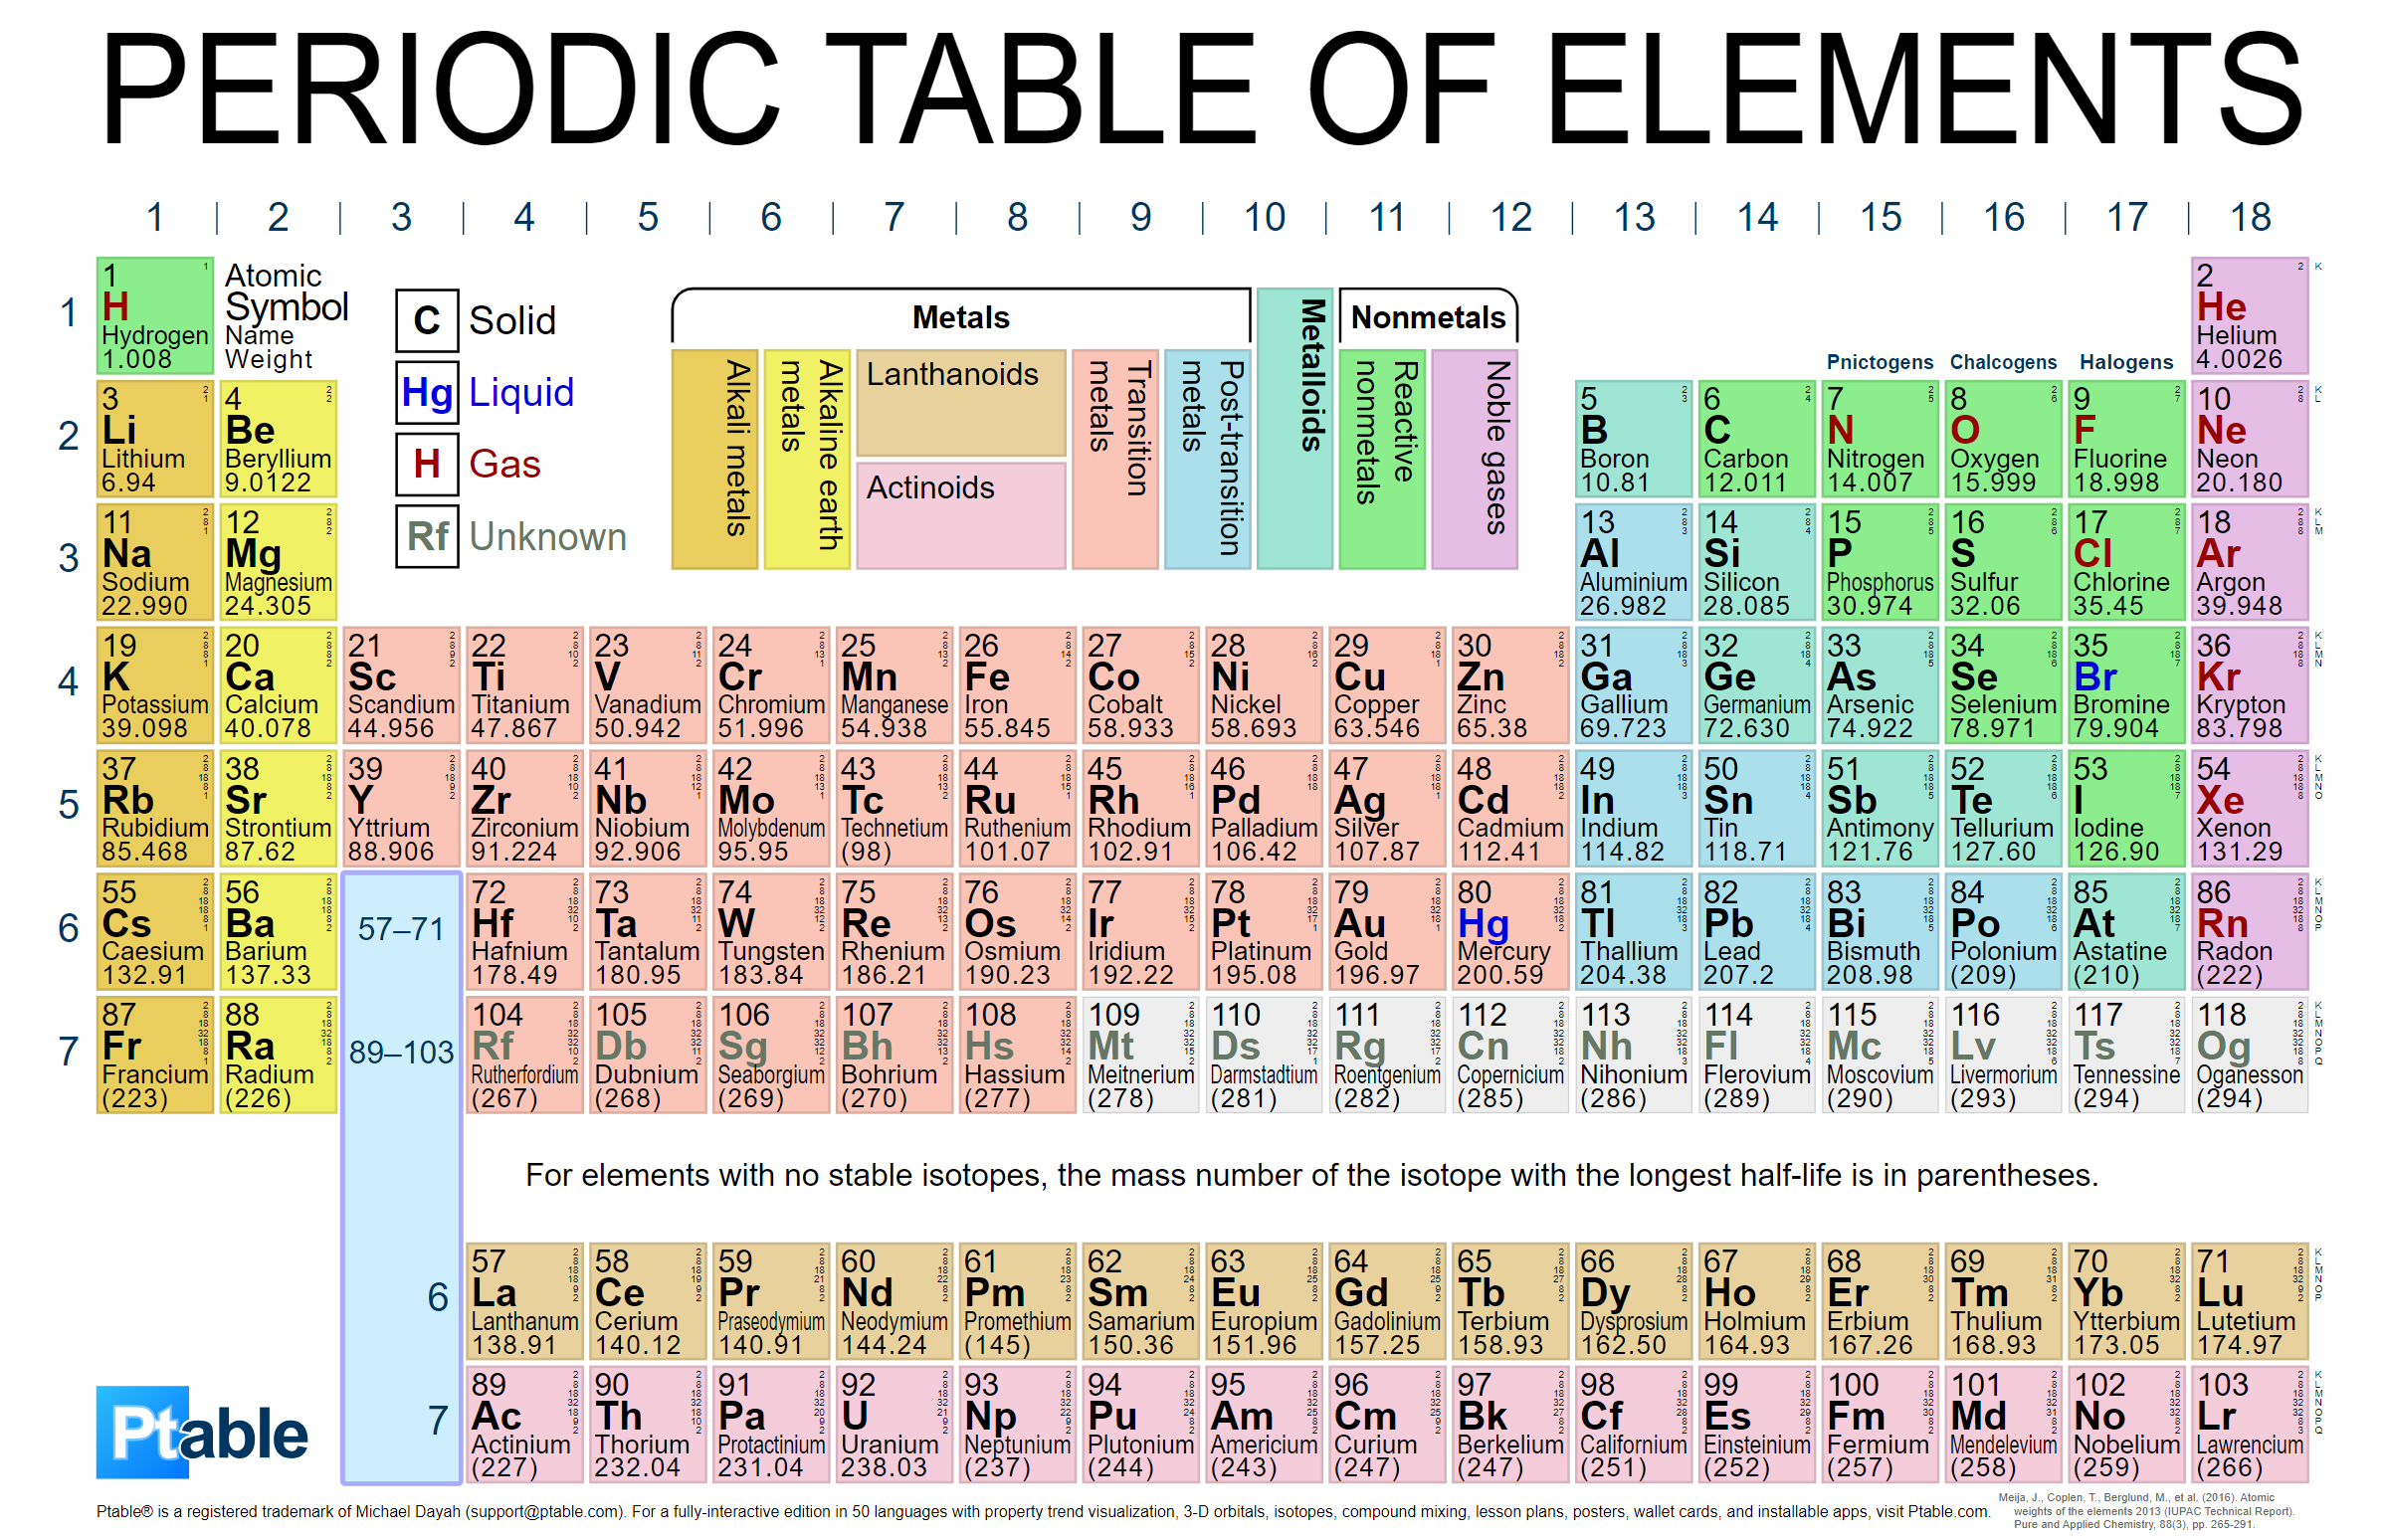
\includegraphics[angle=90,origin=c,width=.629\paperwidth]{img/periodic-table.png}}
    \caption{Periodiska systemet.}
\end{figure}
\vfill
\pagebreak

\section{Formelsamling}
\centering
\begin{table}[h!]
    \def\arraystretch{1.5}
    \centering
    \begin{tabular}{c | c | c}
        \textbf{Konstant} & \textbf{Symbol} & \textbf{Värde} \\ \midrule
        Pi & $\pi$ & \num{3.14159265359} \\
        Ljusets hastighet & $c$ & \SI{299792458}{\m\per\s} \\
        Wiens förskjutningskonstant & $b$ & \SI{2.8977719e-3}{\m\kelvin}
    \end{tabular}
    \caption{Konstanter.}
\end{table}

\begin{table}[h!]
    \def\arraystretch{1.5}
    \centering
    \begin{tabular}{c | c}
        \textbf{Formel} & \textbf{Uttryck} \\ \midrule
        Wiens förskjutningslag & $\displaystyle \lambda_\text{max} = \frac{b}{T}$ \\
        Massa-energiekvivalens & $\displaystyle E = mc^2$
    \end{tabular}
    \caption{Formler.}
\end{table}
\end{document}